\begin{figure}[h]
\centering
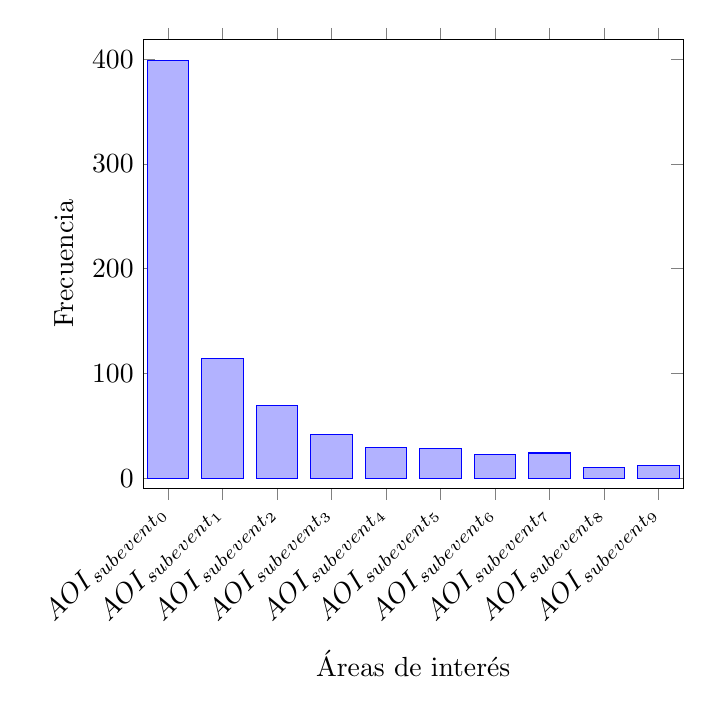
\begin{tikzpicture}
\begin{axis}[
    x tick label style={rotate=45, anchor=east},
    ylabel=Frecuencia,
    xlabel=Áreas de interés,
    enlargelimits=0.05,
    legend style={at={(0.5,-0.1)}, anchor=north,legend columns=-1},
    ybar,
    bar width=15pt,
    symbolic x coords={$\text{AOI}_{subevent_0}$,$\text{AOI}_{subevent_1}$,$\text{AOI}_{subevent_2}$,$\text{AOI}_{subevent_3}$,$\text{AOI}_{subevent_4}$,$\text{AOI}_{subevent_5}$,$\text{AOI}_{subevent_6}$,$\text{AOI}_{subevent_7}$,$\text{AOI}_{subevent_8}$,$\text{AOI}_{subevent_9}$},
    xtick=data
]
\addplot coordinates {
    ($\text{AOI}_{subevent_0}$, 399)
    ($\text{AOI}_{subevent_1}$, 114)
    ($\text{AOI}_{subevent_2}$, 69)
    ($\text{AOI}_{subevent_3}$, 42)
    ($\text{AOI}_{subevent_4}$, 29)
    ($\text{AOI}_{subevent_5}$, 28)
    ($\text{AOI}_{subevent_6}$, 23)
    ($\text{AOI}_{subevent_7}$, 24)
    ($\text{AOI}_{subevent_8}$, 10)
    ($\text{AOI}_{subevent_9}$, 12)
};
\end{axis}
\end{tikzpicture}
\end{figure}